% Localization benchmark in simulation: findings (short report, 6 pages).
% The full 17-page version is main_long.tex.
% Build: latexmk -pdf main.tex   (figures/ and tables/ come from scripts/report_figures.py)
\documentclass[10pt,letterpaper]{article}

% ---------------------------------------------------------------- packages
\usepackage[T1]{fontenc}
\usepackage[utf8]{inputenc}
\usepackage{lmodern}
\usepackage[final]{microtype}
\usepackage[margin=0.75in,top=0.7in,bottom=0.8in]{geometry}
\usepackage{amsmath}
\usepackage{graphicx}
\usepackage[export]{adjustbox}
\usepackage{booktabs}
\usepackage{array}
\usepackage{makecell}
\renewcommand{\theadfont}{\normalsize}
\usepackage{tabularx}
\usepackage[detect-all]{siunitx}
\usepackage{xcolor}
\usepackage{caption}
\usepackage{enumitem}
\usepackage[compact]{titlesec}
\usepackage{placeins}
\usepackage[hidelinks]{hyperref}
\usepackage[capitalise,noabbrev]{cleveref}

% ---------------------------------------------------------------- style
\definecolor{scan}{HTML}{2A78D6}
\definecolor{amcl}{HTML}{EB6834}
\definecolor{slam}{HTML}{1BAF7A}
\definecolor{odom}{HTML}{8F8E89}
\definecolor{ink2}{HTML}{5A5A5A}
\newcommand{\swatch}[1]{\textcolor{#1}{\rule[0.05em]{0.7em}{0.7em}}}
\newcommand{\code}[1]{\texttt{#1}}
\newcommand{\tablenote}[1]{\par\vspace{2pt}{\footnotesize\color{ink2}#1\par}}

\captionsetup{font=small,labelfont=bf,labelsep=period,skip=4pt}
\captionsetup[table]{position=top}
\setlist{itemsep=1pt,topsep=2pt,parsep=0pt,leftmargin=1.3em}
\titlespacing*{\section}{0pt}{8pt}{3pt}
\titlespacing*{\subsection}{0pt}{5pt}{2pt}
\setlength{\textfloatsep}{9pt plus 2pt minus 2pt}
\setlength{\floatsep}{8pt plus 2pt minus 2pt}
\renewcommand{\topfraction}{0.9}
\renewcommand{\bottomfraction}{0.8}
\renewcommand{\textfraction}{0.07}
\renewcommand{\floatpagefraction}{0.8}
\setcounter{topnumber}{3}
\setcounter{bottomnumber}{2}
\setcounter{totalnumber}{5}
\renewcommand{\arraystretch}{1.08}
\sisetup{range-phrase=--,range-units=single}
\pagestyle{plain}

% generated by scripts/report_figures.py: values quoted in the text, used as \val{key}
\makeatletter
\@namedef{val@amcl-filled-p95}{24.5}
\@namedef{val@amcl-n0-lost}{0/3}
\@namedef{val@amcl-n0-rmse}{6.2}
\@namedef{val@amcl-n0-yaw}{1.2}
\@namedef{val@amcl-n1-lost}{0/3}
\@namedef{val@amcl-n1-rmse}{9.4}
\@namedef{val@amcl-n1-yaw}{1.9}
\@namedef{val@amcl-n2-lost}{0/3}
\@namedef{val@amcl-n2-rmse}{13.4}
\@namedef{val@amcl-n2-yaw}{2.7}
\@namedef{val@amcl-n4-lost}{1/3}
\@namedef{val@amcl-n4-rmse}{23.7}
\@namedef{val@amcl-n4-yaw}{4.4}
\@namedef{val@amcl-n8-lost}{3/3}
\@namedef{val@amcl-n8-rmse}{36.5}
\@namedef{val@amcl-n8-yaw}{6.7}
\@namedef{val@amcl-outline-lost}{0/17}
\@namedef{val@amcl-outline-p95}{11.2}
\@namedef{val@amcl-outline-rmse}{6.3}
\@namedef{val@amcl-outline-yaw}{1.1}
\@namedef{val@amcl-sweep-lost}{6/17}
\@namedef{val@amcl-sweep-rmse}{12.4}
\@namedef{val@amcl-sweep-yaw}{2.6}
\@namedef{val@noise-rtf-max}{1.00}
\@namedef{val@noise-rtf-min}{0.85}
\@namedef{val@odom-n0-lost}{0/3}
\@namedef{val@odom-n0-rmse}{0.0}
\@namedef{val@odom-n0-yaw}{0.0}
\@namedef{val@odom-n1-lost}{3/3}
\@namedef{val@odom-n1-rmse}{2.2}
\@namedef{val@odom-n1-yaw}{24.5}
\@namedef{val@odom-n2-lost}{3/3}
\@namedef{val@odom-n2-rmse}{4.2}
\@namedef{val@odom-n2-yaw}{48.9}
\@namedef{val@odom-n4-lost}{3/3}
\@namedef{val@odom-n4-rmse}{6.9}
\@namedef{val@odom-n4-yaw}{97.8}
\@namedef{val@odom-n8-lost}{3/3}
\@namedef{val@odom-n8-rmse}{7.6}
\@namedef{val@odom-n8-yaw}{101}
\@namedef{val@runs-noise}{60}
\@namedef{val@scan-n0-lost}{0/3}
\@namedef{val@scan-n0-rmse}{4.0}
\@namedef{val@scan-n0-yaw}{0.5}
\@namedef{val@scan-n1-lost}{0/3}
\@namedef{val@scan-n1-rmse}{4.3}
\@namedef{val@scan-n1-yaw}{0.6}
\@namedef{val@scan-n2-lost}{0/3}
\@namedef{val@scan-n2-rmse}{4.6}
\@namedef{val@scan-n2-yaw}{0.6}
\@namedef{val@scan-n4-lost}{0/3}
\@namedef{val@scan-n4-rmse}{5.3}
\@namedef{val@scan-n4-yaw}{0.9}
\@namedef{val@scan-n8-lost}{0/3}
\@namedef{val@scan-n8-rmse}{11.6}
\@namedef{val@scan-n8-yaw}{2.6}
\@namedef{val@scan-sweep-lost}{0/17}
\@namedef{val@scan-sweep-rmse}{5.1}
\@namedef{val@scan-sweep-yaw}{0.6}
\@namedef{val@slam-fixed-lost}{0/15 (+2 failed)}
\@namedef{val@slam-fixed-p95}{8.0}
\@namedef{val@slam-fixed-rmse}{5.2}
\@namedef{val@slam-fixed-rtf-max}{0.99}
\@namedef{val@slam-fixed-rtf-min}{0.53}
\@namedef{val@slam-fixed-yaw}{0.7}
\@namedef{val@slam-lc-off-max}{8.6}
\@namedef{val@slam-lc-off-rmse}{5.0}
\@namedef{val@slam-lc-on-max}{145}
\@namedef{val@slam-lc-on-rmse}{47.0}
\@namedef{val@slam-n0-lost}{0/3}
\@namedef{val@slam-n0-rmse}{5.2}
\@namedef{val@slam-n0-yaw}{0.8}
\@namedef{val@slam-n1-lost}{0/3}
\@namedef{val@slam-n1-rmse}{5.0}
\@namedef{val@slam-n1-yaw}{0.6}
\@namedef{val@slam-n2-lost}{0/3}
\@namedef{val@slam-n2-rmse}{5.0}
\@namedef{val@slam-n2-yaw}{0.6}
\@namedef{val@slam-n4-lost}{0/3}
\@namedef{val@slam-n4-rmse}{5.3}
\@namedef{val@slam-n4-yaw}{0.8}
\@namedef{val@slam-n8-lost}{0/3}
\@namedef{val@slam-n8-rmse}{7.3}
\@namedef{val@slam-n8-yaw}{1.6}
\@namedef{val@slam-ref-off-max}{22.1}
\@namedef{val@slam-ref-off-rmse}{9.5}
\@namedef{val@slam-ref-on-max}{213}
\@namedef{val@slam-ref-on-rmse}{86.6}
\@namedef{val@slam-sweep-lost}{17/17}
\@namedef{val@slam-sweep-rmse}{92.9}
\@namedef{val@slam-sweep-yaw}{7.9}
\@namedef{val@victoria_ref-rest-within10}{93}
\@namedef{val@victoria_ref-start-within10}{74}
\@namedef{val@victoria_ref_lc-rest-within10}{86}
\@namedef{val@victoria_ref_lc-start-within10}{91}
\newcommand{\val}[1]{\@ifundefined{val@#1}{\textbf{??}}{\@nameuse{val@#1}}}
\makeatother


\begin{document}

\begin{center}
  {\LARGE\bfseries Localization in Simulation: AMCL, SLAM Toolbox and a Scan Matcher}\\[5pt]
  {\large Ingenuity Labs Localization Team}\\[2pt]
  {\small\color{ink2}22 November 2026}
\end{center}

\noindent\textbf{Summary.}
We compared three 2D lidar localizers for our F1TENTH car in a Gazebo simulation of the Victoria
track. A speed sweep with perfect odometry showed that only our scan matcher worked as configured:
AMCL lost track in \val{amcl-sweep-lost} runs and SLAM Toolbox in \val{slam-sweep-lost}. Both causes
were configuration problems. AMCL scored lidar beams against a map whose off-track area is filled
in; on a walls-only map its error halved (\SI{\val{amcl-sweep-rmse}}{} $\to$
\SI{\val{amcl-outline-rmse}}{cm}) and it no longer lost track. SLAM Toolbox re-optimized its whole
map on wrong loop closures during localization; with loop closure off it went from
\SI{\val{slam-sweep-rmse}}{} to \SI{\val{slam-fixed-rmse}}{cm}. With perfect odometry all three then
reach \SIrange{4}{6}{cm}, so we repeated the test with simulated odometry error: SLAM Toolbox was
the most robust, the scan matcher the most accurate at low noise, and AMCL degraded steadily until it
lost track.

% =====================================================================
\section{Setup and methods}\label{sec:setup}

\textbf{Simulation.} The Gazebo world is generated from the race stack's Victoria occupancy map, so
the Gazebo frame equals the map frame. The differential-drive car carries a lidar similar to a Hokuyo
UST-10LX (\ang{270}, 1081 beams, \SI{40}{Hz}, range noise $\sigma=\SI{1}{cm}$). Odometry is
Gazebo's exact pose unless the noise of \cref{sec:noise} is switched on; ground truth is always
exact. An autopilot follows the centerline (\SI{36.8}{m} per lap) and steers on ground truth, so every
localizer sees the same drive.

\begin{table}[htbp]
  \centering\small
  \caption{The three localizers in their final configuration.}
  \label{tab:localizers}
  \begin{tabularx}{\linewidth}{@{}>{\raggedright\arraybackslash}p{1.6cm}>{\raggedright\arraybackslash}X
                                >{\raggedright\arraybackslash}X>{\raggedright\arraybackslash}X@{}}
    \toprule
    & \swatch{scan}~Scan matcher (ours) & \swatch{amcl}~AMCL (Nav2~\cite{macenski2020marathon}) &
      \swatch{slam}~SLAM Toolbox 2.6~\cite{macenski2021slam} \\
    \midrule
    Map & fixed image, walls only & fixed image, walls only & own pose graph, recorded in the sim \\
    Method & per scan: odometry prediction, Gauss--Newton fit of every 4th beam to a distance field,
        weak odometry prior & particle filter~\cite{thrun2005probabilistic,fox2003kld}, 500--2000
        particles, likelihood field, 60 beams & matches each scan against its recent scans and nearby
        map scans (Karto), weighted mean \\
    Updates & every scan (\SI{40}{Hz}) & every \SI{0.1}{m} or \SI{0.1}{rad} & every \SI{0.1}{m} or
        \SI{0.1}{rad} \\
    When lost & no recovery (searches \SI{\pm0.5}{m}) & no recovery (disabled) & no recovery (window
        \SI{\pm0.25}{m}) \\
    \bottomrule
  \end{tabularx}
\end{table}

\textbf{Localizers} (\cref{tab:localizers}). AMCL and the scan matcher localize on a fixed map image;
SLAM Toolbox cannot load an image and uses a pose graph it recorded in the simulation. The maps are
idealized: AMCL and the scan matcher get exactly the wall pixels the simulated walls were built from,
and SLAM Toolbox's map was recorded with a matcher constrained to the perfect odometry. The absolute
numbers are therefore upper bounds for maps from a real mapping run.

\textbf{Procedure and metrics.} Each run starts a fresh simulation and one localizer in its own
Gazebo partition and ROS domain, so runs execute in parallel without interfering. For every
ground-truth message, an error node compares the true pose with the localizer's estimate at exactly
the same timestamp. All metrics cover the driving window only: \emph{position RMSE} (typical error),
\emph{p95} (the bad moments), \emph{heading RMSE}, and \emph{lost track} (error above \SI{0.5}{m} at
any point, about a third of the track width). Tables report medians over runs.

% =====================================================================
\section{Speed sweep}\label{sec:sweep}

\textbf{Design and rationale.} Each localizer drove one 3-lap run at each of 17 speeds from 0.20 to
\SI{1.00}{m/s} (51 runs, 82 minutes on 3 parallel workers), with perfect odometry so that only the
localizer varied. One run at many speeds replaces repeated runs at a few: with no speed dependence,
neighbouring speeds act as repeats, and with one, the trend becomes visible. Three laps per run pass
every point of the track three times, which separates errors tied to a place from random ones and
shows whether a localizer recovers.

\begin{figure}[htbp]
  \centering
  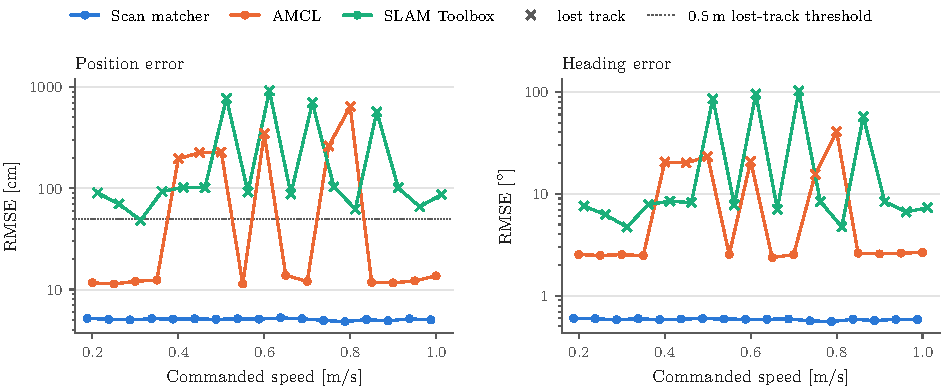
\includegraphics[max width=\linewidth]{figures/speed_sweep.pdf}
  \caption{Original speed sweep: every run's position and heading RMSE over commanded speed (log
  scales). Crosses: runs that lost track. The scan matcher is flat at \SI{5}{cm}; AMCL alternates
  between about \SI{12}{cm} and lost runs; SLAM Toolbox loses track at every speed.}
  \label{fig:sweep}
\end{figure}

\begin{figure}[htbp]
  \centering
  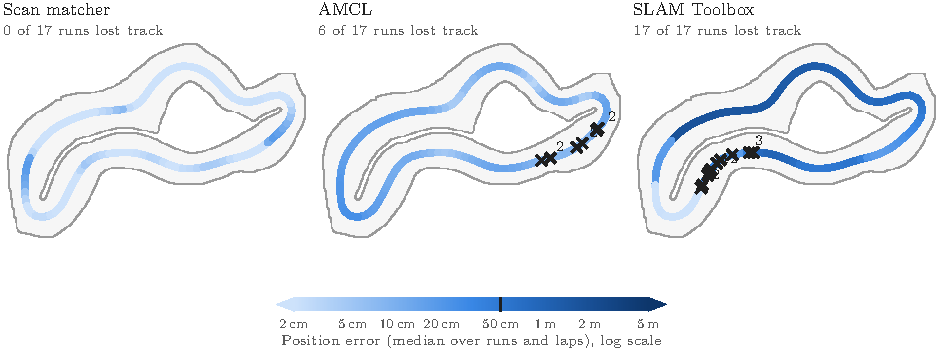
\includegraphics[max width=\linewidth]{figures/speed_sweep_track.pdf}
  \caption{Where the original configurations failed: median error along the lap over all runs and
  laps, and where each run first exceeded \SI{0.5}{m} (numbers: runs per cluster). AMCL fails on the
  way into the hairpin (right), SLAM Toolbox a few metres after the start (bottom left).}
  \label{fig:track}
\end{figure}

\textbf{Results} (\cref{fig:sweep,fig:track}). The scan matcher reached
\SI{\val{scan-sweep-rmse}}{cm} and \ang{\val{scan-sweep-yaw}} at every speed and never lost track.
AMCL reached about \SI{12}{cm} in its good runs but lost track in \val{amcl-sweep-lost}, each time
with a sudden jump of 2.7--4.3\,m on the way into the hairpin. SLAM Toolbox failed in all
\val{slam-sweep-lost} runs at the same place, 2.5--3.5\,m after the start, and recovered partly each
time it passed the start line. The sweep taught us three things:
\begin{itemize}
  \item No localizer depends on speed in this range; the failures are tied to places, which pointed
        the diagnosis at the maps (\cref{sec:fixes}).
  \item With perfect odometry nothing accumulates: the scan matcher's error is the same in every lap.
  \item With perfect odometry and a correct start, a localizer that did nothing would score zero. The
        sweep measures how much a localizer \emph{disturbs} good odometry, not how well it
        \emph{corrects} bad odometry, which motivated the noise test (\cref{sec:noise}).
\end{itemize}

% =====================================================================
\FloatBarrier
\section{Fixing AMCL and SLAM Toolbox}\label{sec:fixes}

\subsection{AMCL: the map}

AMCL weights particles with a likelihood field: each beam endpoint contributes
$p_\mathrm{hit}=\exp(-d^2/2\sigma^2)$, where $d$ is the distance to the nearest occupied map cell
($\sigma=\SI{0.2}{m}$). The race stack's Victoria map is \emph{filled}: the whole off-track area is
occupied, 67\,\% of all pixels. There $d=0$, so a beam that passes a wall and ends behind it still
scores a perfect hit (\cref{fig:amcl-maps}). A particle shifted outwards loses almost nothing, the
weights flatten in exactly the direction the car can be wrong, and the estimate can jump. In the lost
runs the estimate jumped several metres within a second and then followed a shifted copy of the path,
largely inside the occupied area.

\begin{figure}[htbp]
  \centering
  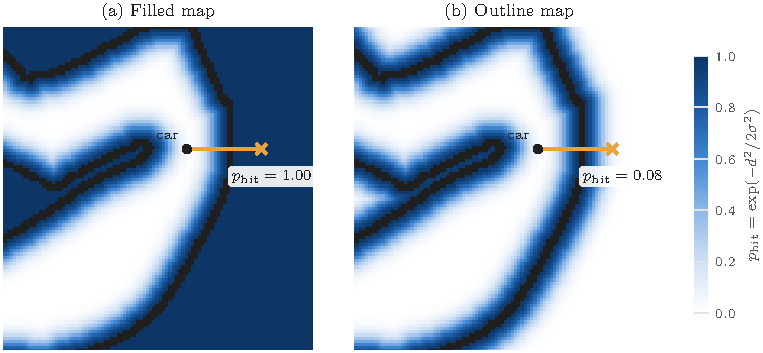
\includegraphics[max width=\linewidth]{figures/amcl_maps_compact.pdf}
  \caption{AMCL's likelihood-field hit term in the hairpin; the beam from the car ends \SI{0.4}{m}
  behind the outer wall. (a)~Filled map: every off-track cell is occupied, so the beam still scores
  $p_\mathrm{hit}=1$. (b)~Outline map: only the walls are occupied and the same beam scores
  near zero. Inside the track the two fields are identical.}
  \label{fig:amcl-maps}
\end{figure}

\textbf{Fix.} A small tool (\code{outline\_map}) keeps only the occupied pixels that touch free
space, the same rule the world generator uses, and marks the rest unknown (\num{3829} of \num{54384}
occupied pixels remain). On this map AMCL lost no run, and its median RMSE halved from
\SI{\val{amcl-sweep-rmse}}{cm} to \SI{\val{amcl-outline-rmse}}{cm}, with heading error falling from
\ang{\val{amcl-sweep-yaw}} to \ang{\val{amcl-outline-yaw}} (\cref{fig:fixes}a, \cref{tab:sweep}). The
gain in runs that never lost track shows that the filled map also blurred normal operation.

\subsection{SLAM Toolbox: loop closure in localization mode}

SLAM Toolbox's failures were jumps near the start, and its reference map had doubled walls there,
offset by 10--15\,cm: it had been recorded with loop closure off, so the drift of the mapping lap
(\SI{28}{cm}, \ang{2.5}) remained where the lap ended. Re-recording the map with loop closure fixed
the walls (\val{victoria_ref_lc-start-within10}\,\% of wall pixels in the start area within
\SI{10}{cm} of the true wall, up from \val{victoria_ref-start-within10}\,\%), but localization
\emph{still failed at the same place} (\cref{tab:slam-variants}).

\begin{table}[htbp]
  \centering\small
  \caption{SLAM Toolbox at \SI{1.0}{m/s}: map $\times$ loop closure in localization mode.}
  \label{tab:slam-variants}
  \begin{tabular}{llrrrrrr}
\toprule
Map & \makecell[lb]{{Loop} \\ {closure}} & \makecell[rb]{{RMSE} \\ {[cm]}} & \makecell[rb]{{p95} \\ {[cm]}} & \makecell[rb]{{Max} \\ {[cm]}} & \makecell[rb]{{Heading} \\ {RMSE [$^\circ$]}} & \makecell[rb]{{Heading} \\ {max [$^\circ$]}} & Laps \\
\midrule
\texttt{victoria\_ref} & on & 86.6 & 180 & 213 & 7.3 & 24.6 & 3 \\
\texttt{victoria\_ref\_lc} & on & 47.0 & 109 & 145 & 3.8 & 16.1 & 1 \\
\texttt{victoria\_ref} & off & 9.5 & 20.2 & 22.1 & 1.1 & 3.0 & 1 \\
\texttt{victoria\_ref\_lc} & off & 5.0 & 7.7 & 8.6 & 0.7 & 2.1 & 1 \\
\bottomrule
\end{tabular}

  \tablenote{First row: the 3-lap run of the original sweep; the others are single laps.}
\end{table}

The cause is in the localization mode itself. For each scan, SLAM Toolbox (Karto) matches against its
recent scans and the nearby map scans, and then tries to close a loop against other map scans within
\SI{3}{m}. A successful loop closure (\code{TryCloseLoop}) calls \code{CorrectPoses}, which
re-optimizes the \emph{entire} pose graph, including the saved map. A wrong match near the start
therefore moves both the pose and the map, and later scans are matched against a distorted map.
Turning loop closure off reduced the error ninefold on the old map, and the clean map halved what
remained (\cref{tab:slam-variants}). The trade-off: without loop closure SLAM Toolbox cannot
re-localize once its error exceeds its search window of about \SI{\pm0.25}{m}, a limitation the other
two share. The full sweep confirmed the fix: \SI{\val{slam-fixed-rmse}}{cm}, flat over speed, no run
lost (\cref{fig:fixes}b).\footnote{Two runs of this sweep are missing because a benchmark bug blocked
their start (since fixed). The six parallel instances slowed the simulation to down to 0.53 of real
time, which gives SLAM Toolbox more computer time than on the car; a single run at full speed gave
the same \SI{5}{cm}.}

\begin{figure}[htbp]
  \centering
  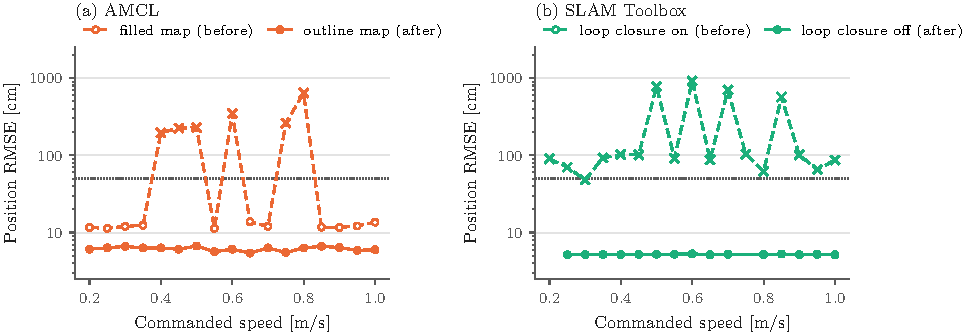
\includegraphics[max width=\linewidth]{figures/fixes_before_after.pdf}
  \caption{Both fixes over speed: position RMSE before (dashed, open circles) and after (solid);
  crosses mark lost runs, the dotted line is the \SI{0.5}{m} lost-track threshold. After the fixes no
  run lost track and both errors are flat over speed.}
  \label{fig:fixes}
\end{figure}

\begin{table}[htbp]
  \centering\small
  \caption{Speed sweeps before and after the fixes: medians over the runs at 17 speeds (3 laps
  each). After the fixes all three are within \SIrange{4}{6}{cm}.}
  \label{tab:sweep}
  \begin{tabular}{llrrrr}
\toprule
\makecell[lb]{{Localizer}} & \makecell[lb]{{Configuration}} & \makecell[rb]{{RMSE} \\ {[cm]}} & \makecell[rb]{{p95} \\ {[cm]}} & \makecell[rb]{{Heading} \\ {RMSE [$^\circ$]}} & \makecell[rb]{{Lost} \\ {track}} \\
\midrule
Scan matcher & filled map & 5.1 & 13.9 & 0.6 & 0/17 \\
\midrule
AMCL & filled map (before) & 12.4 & 24.5 & 2.6 & 6/17 \\
 & outline map (after) & 6.3 & 11.2 & 1.1 & 0/17 \\
\midrule
SLAM Toolbox & loop closure on, \texttt{victoria\_ref} (before) & 92.9 & 180 & 7.9 & 17/17 \\
 & loop closure off, \texttt{victoria\_ref\_lc} (after) & 5.2 & 8.0 & 0.7 & 0/15 (+2 failed) \\
\bottomrule
\end{tabular}

  \tablenote{The scan matcher's sweep used the filled map; on the outline map it reached
  \SI{\val{scan-n0-rmse}}{cm} at \SI{1.0}{m/s} (\cref{tab:noise}, level 0).}
\end{table}

\Cref{fig:heatmap-fixes} shows the improvement along the track, with one row per run and the three
laps side by side, so that a column is the same place in every lap. Before the fixes, each AMCL
failure is a dark band that starts on the way into the hairpin and either lasts to the end of the run
or ends when the filter happens to snap back; SLAM Toolbox goes dark a few metres after the start in
every run and recovers only briefly near the start line. After the fixes both are light everywhere.
SLAM Toolbox's small remaining error rises slightly after the hairpin and in the left-hand corner, in
the same places in every run, while AMCL's is spread evenly along the lap.

\begin{figure}[htbp]
  \centering
  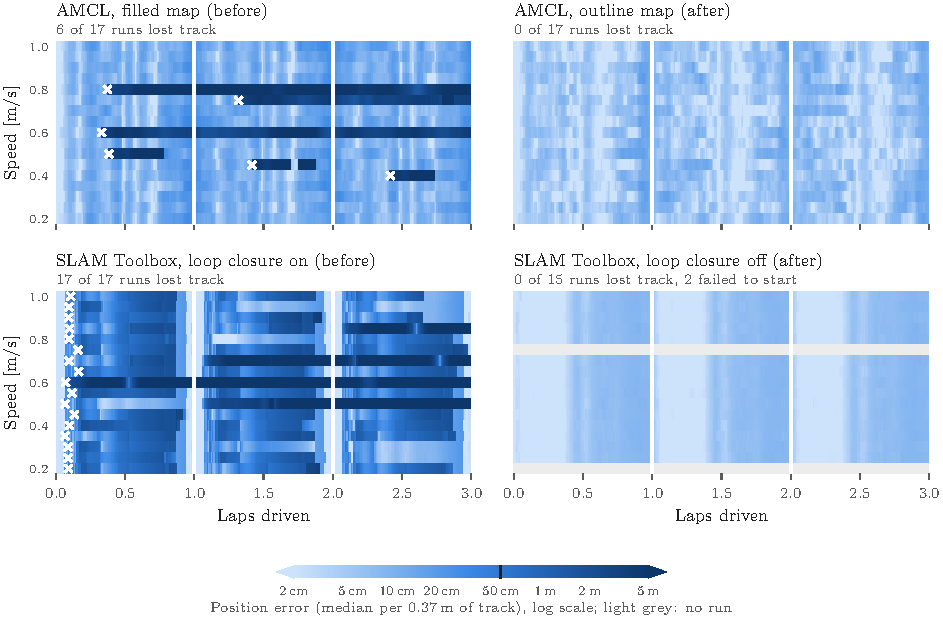
\includegraphics[max width=\linewidth]{figures/heatmap_fixes.pdf}
  \caption{Error along the three laps before (left) and after (right) each fix: one row per run
  (speed), one cell per \SI{0.37}{m} of track, white lines at the start of each lap. Crosses mark where
  a run first exceeded \SI{0.5}{m}. The two empty rows on the bottom right are the runs that failed to
  start.}
  \label{fig:heatmap-fixes}
\end{figure}

% =====================================================================
\FloatBarrier
\section{Odometry noise test}\label{sec:noise}

\textbf{Noise model.} On the car, odometry from the motor controller and IMU drifts, and removing that
drift is the localizer's job. A node between the simulator and the localizers corrupts each
\SI{50}{Hz} odometry step and integrates the result from the true start pose. At \emph{level 1}, our
estimate of a real car, distances read \SI{2}{\%} long, turns \SI{2}{\%} too sharp, the gyroscope has
a bias of \SI{0.2}{\degree/s}, and a random walk adds \SI{1}{cm} and \ang{0.3} per
$\sqrt{\mathrm{m}}$ driven; level $k$ multiplies every term by $k$. At level 1 the odometry alone is
already about \SI{1.5}{m} and \ang{10}--\ang{13} off after one lap. Level 1 is an estimate, not a
measurement from our car.

\textbf{Design.} All three localizers plus an \emph{odometry only} reference (no localizer, so its
error is the raw drift) ran at levels 0, 1, 2, 4 and 8, with three runs per level at \SI{1.0}{m/s}
(3 laps each; \val{runs-noise} runs in 31 minutes). Run $r$ of every localizer used noise seed $r$,
so all received the same corrupted odometry. Speed was fixed because the sweep showed no speed
dependence; the three seeds replace it as repeats.

\begin{figure}[htbp]
  \centering
  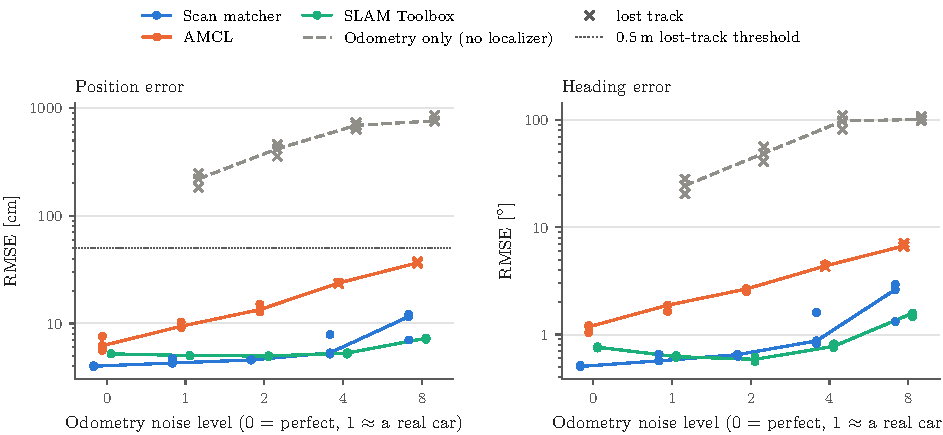
\includegraphics[max width=\linewidth]{figures/noise_rmse.pdf}
  \caption{Position and heading RMSE over odometry noise level (log scales); one dot per run, lines
  through the medians. Dashed grey: the odometry alone (zero at level 0, not drawn).}
  \label{fig:noise}
\end{figure}

\begin{table}[htbp]
  \centering\small
  \setlength{\tabcolsep}{3.6pt}
  \caption{Noise test, medians over three runs per level. RMSE and p95 in cm, heading (Hdg) RMSE in
  degrees, lost = runs above \SI{0.5}{m}.}
  \label{tab:noise}
  \begin{tabular}{crrrrrrrrrrrrr}
\toprule
 & \multicolumn{4}{c}{Scan matcher} & \multicolumn{4}{c}{AMCL} & \multicolumn{4}{c}{SLAM Toolbox} & Odom. only \\
\cmidrule(lr){2-5}\cmidrule(lr){6-9}\cmidrule(lr){10-13}\cmidrule(lr){14-14}
Level & RMSE & p95 & Hdg & Lost & RMSE & p95 & Hdg & Lost & RMSE & p95 & Hdg & Lost & RMSE [m] \\
\midrule
0 & 4.0 & 9.9 & 0.5 & 0/3 & 6.2 & 11.8 & 1.2 & 0/3 & 5.2 & 7.9 & 0.8 & 0/3 & 0 \\
1 & 4.3 & 10.6 & 0.6 & 0/3 & 9.4 & 16.1 & 1.9 & 0/3 & 5.0 & 7.9 & 0.6 & 0/3 & 2.20 \\
2 & 4.6 & 10.9 & 0.6 & 0/3 & 13.4 & 23.3 & 2.7 & 0/3 & 5.0 & 7.8 & 0.6 & 0/3 & 4.19 \\
4 & 5.3 & 11.8 & 0.9 & 0/3 & 23.7 & 36.7 & 4.4 & 1/3 & 5.3 & 8.4 & 0.8 & 0/3 & 6.90 \\
8 & 11.6 & 20.4 & 2.6 & 0/3 & 36.5 & 61.4 & 6.7 & 3/3 & 7.3 & 12.3 & 1.6 & 0/3 & 7.62 \\
\bottomrule
\end{tabular}

\end{table}

\textbf{Results} (\cref{fig:noise}, \cref{tab:noise}).
\begin{itemize}
  \item \swatch{slam}~\textbf{SLAM Toolbox} was the most robust: \SI{\val{slam-n0-rmse}}{cm} with
        perfect odometry, \SI{\val{slam-n4-rmse}}{cm} at level 4 and \SI{\val{slam-n8-rmse}}{cm} at
        level 8, never lost, with the least spread between seeds.
  \item \swatch{scan}~\textbf{The scan matcher} was the most accurate up to level 2 and level with
        SLAM Toolbox at level 4 (\SI{\val{scan-n4-rmse}}{cm}), but roughly doubled its error at level 8
        (\SI{\val{scan-n8-rmse}}{cm}). It never lost track.
  \item \swatch{amcl}~\textbf{AMCL}'s error grew with every level, from \SI{\val{amcl-n0-rmse}}{cm} to
        \SI{\val{amcl-n8-rmse}}{cm}. It lost track in \val{amcl-n4-lost} runs at level 4 and
        \val{amcl-n8-lost} at level 8, with worst errors of 0.4--\SI{1.0}{m} rather than the
        multi-metre jumps of the filled map.
  \item \swatch{odom}~\textbf{The odometry alone} was \SI{\val{odom-n1-rmse}}{m} off at level 1 and
        \SI{\val{odom-n8-rmse}}{m} at level 8; all three localizers removed most of it.
\end{itemize}
These differences fit how the methods work, although we have not tested the explanations separately:
AMCL spreads its particles by a fixed fraction of each odometry step and corrects them with flat
weights, so a systematic error is only partly removed; the scan matcher refines from the odometry
prediction with a local fit, which works until the error between scans grows large; SLAM Toolbox
first searches a grid of poses around the prediction, which tolerates larger errors.

% =====================================================================
\section{Conclusions}\label{sec:conclusions}

\begin{itemize}
  \item The speed sweep found no speed dependence; its value was in locating the failures, which were
        configuration problems, not algorithmic limits.
  \item AMCL must use a walls-only map: on a filled map, beams behind walls count as hits.
  \item SLAM Toolbox must run with loop closure off in localization mode, on a map recorded with loop
        closure: in localization, loop closure re-optimizes and moves the map.
  \item With perfect odometry all three reach \SIrange{4}{6}{cm}; under odometry noise SLAM Toolbox is
        the most robust, the scan matcher the most accurate at low noise, and AMCL the least robust.
\end{itemize}

{\small
\begin{thebibliography}{9}\setlength{\itemsep}{0pt}
\bibitem{macenski2021slam}
S.~Macenski and I.~Jambrecic, ``SLAM Toolbox: SLAM for the dynamic world,'' \emph{Journal of Open
Source Software}, vol.~6, no.~61, p.~2783, 2021.
\bibitem{macenski2020marathon}
S.~Macenski, F.~Mart\'in, R.~White, and J.~Gin\'es Clavero, ``The Marathon 2: A navigation
system,'' in \emph{Proc.\ IEEE/RSJ IROS}, 2020.
\bibitem{thrun2005probabilistic}
S.~Thrun, W.~Burgard, and D.~Fox, \emph{Probabilistic Robotics}. MIT Press, 2005.
\bibitem{fox2003kld}
D.~Fox, ``Adapting the sample size in particle filters through KLD-sampling,'' \emph{Int.\ J.\
Robotics Research}, vol.~22, no.~12, pp.~985--1003, 2003.
\end{thebibliography}}

\end{document}
